%% The first command in your LaTeX source must be the \documentclass command.
%%
%% Options:
%% twocolumn : Two column layout.
%% hf: enable header and footer.
\documentclass[
% twocolumn,
% hf,
]{ceurart}

%%
%% One can fix some overfulls
\sloppy

%%
%% Minted listings support 
%% Need pygment <http://pygments.org/> <http://pypi.python.org/pypi/Pygments>
\usepackage{listings}
%% auto break lines
\lstset{breaklines=true}


%%%%%%%%%%%%  additional packages  %%%%%
\usepackage{LOA-template}
\usepackage{subcaption}
\usepackage{graphicx}
%%%%%%%%%%%%  -------------------  %%%%%

%%
%% end of the preamble, start of the body of the document source.
\begin{document}

%%
%% Rights management information.
%% CC-BY is default license.
\copyrightyear{2022}
\copyrightclause{Copyright for this paper by its authors.
  Use permitted under Creative Commons License Attribution 4.0
  International (CC BY 4.0).}

%%
%% This command is for the conference information
\conference{\TODO{FOMI 2022: 12th International Workshop on Formal Ontologies meet Industry, held [quando?] [dove?] % held at JOWO 2021: Episode VII The Bolzano Summer of Knowledge, September 11–18 , 2021, Bolzano, Italy
}}

%%
%% The "title" command
\title{Typical problems in functional modelling: a comparison of different approaches}

\tnotemark[1]
\tnotetext[1]{You can use this document as the template for preparing your
  publication. We recommend using the latest version of the ceurart style.}

%%
%% The "author" command and its associated commands are used to define
%% the authors and their affiliations.
\author[1,2]{Dmitry S. Kulyabov}[%
orcid=0000-0002-0877-7063,
email=kulyabov-ds@rudn.ru,
url=https://yamadharma.github.io/,
]
\cormark[1]
\fnmark[1]
\address[1]{ISTC-CNR Laboratory for Applied Ontology, via alla cascata 56/C, 38123, Povo, Italy}
\address[2]{Adige S.P.A, via per Barco, 11, Levico Terme, 38056, Italy}

\author[1]{Ilaria Tiddi}[%
orcid=0000-0001-7116-9338,
email=i.tiddi@vu.nl,
url=https://kmitd.github.io/ilaria/,
]
\fnmark[1]

\author[1]{Manfred Jeusfeld}[%
orcid=0000-0002-9421-8566,
email=Manfred.Jeusfeld@acm.org,
url=http://conceptbase.sourceforge.net/mjf/,
]
\fnmark[1]

%% Footnotes
\cortext[1]{Corresponding author.}
\fntext[1]{These authors contributed equally.}

%%
%% The abstract is a short summary of the work to be presented in the
%% article.
\begin{abstract}
  Functional modelling is a well-studied topic in engineering, biology, and other disciplines. 
  In particular, functional modelling is an essential part of describing engineering systems.
  %Therefore, research on functionality is of interest for applications. <--FC: frase insulsa
  Despite this, functional modelling is seldom and erratically used in industry, as it is difficult to apply consistently in practice.
  As digitalisation becomes an increasingly important necessity in engineering enterprises, this obstacle becomes especially painful.
  In order to attempt to ease such a difficulty, in this paper we analyze two typical problems that are encountered when modelling engineering systems, which are intertwined with functional aspects: permanence of identity of systems components, and granularity management of the models.
  In the paper, those problems are explained, then we compare some possible ontological and engineering approaches that can deal with them.
  Finally, we illustrate our findings in a brief use case.
  \TODO{[S: va sistemato]}
\end{abstract}

%%
%% Keywords. The author(s) should pick words that accurately describe
%% the work being presented. Separate the keywords with commas.
\begin{keywords}
  Functional modelling \sep
  Functional decomposition \sep
  Replacement problem \sep
  Granularity
  %% diachronic identity permanence %\TODO{[?]}
\end{keywords}

%%
%% This command processes the author and affiliation and title
%% information and builds the first part of the formatted document.
\maketitle

%% TODO "theory" --> "ontology"?

\section{Introduction}
    
Functionality is an essential concept in engineering and functional modelling has received widespread attention in the literature. 
Unfortunately, though several theories of functionality have been proposed, no unique treatment has emerged, and some problems persist. In particular, the consistent application of functional modelling is known to be difficult \cite{eckertThatWhichNot2013}.
In this paper, we describe some of the problems that current theories face and\myComment{, building on previous work, <--FC:no, perché sarebbe quello per SWJ} we show, using a brief use case\TODO{<--check}, possible ways to tackle them through applied ontology principles. 

%% introduction & very brief review
\section{Some brief points from the literature}\label{sec:literature}

Functionality is a well-studied topic in engineering \cite{chandrasekaranFunctionalRepresentationDesign1993, umedaFunctionBehaviourStructure1990, hirtz_functional_2002} and ontology \cite{sasajimaFBRLFunctionBehavior1995, TowardAUnifiedDefinition2012}, at least from more than 50 years \cite{collinsFailureExperienceMatrixUseful1976,pahl_engineering_2007} (see also \cite{erdenReviewFunctionModeling2008} for an in-depth review of some aspects of the function-related literature).
We recall very briefly the main characteristics of some theories (or methodologies) of functionality that have been developed in engineering until today.

\begin{itemize}
    \item \textbf{Functional Basis} \cite{hirtz_functional_2002,stone_development_2000}: this methodology considers functions as black-boxes that operate transformations on inputs, producing outputs. The Functional Basis is a vocabulary for functions (e.g., `convert', `distribute') and inputs/outputs (called flows, e.g., `pressure', `electric energy'). The vocabulary is organized in three levels of increasing specialisation. A functional model is a graph whose nodes are boxes and whose edges are arrows labeled with functions and flows terms respectively, which describes the transformations that the flows that enter an engineering system undertake.
    \item \textbf{Functional Representation} \cite{chandrasekaranFunctionalRepresentationDesign1993}: this methodology requires to, first, build a structural model of the system, which is modelled as a set of devices, each one with a set of relevant parameters and input/output ports, and of relations between devices, such as the connection between two ports or the containment of one device into another. Then, state variables are attributed to the system and used to determine different system states. Lastly, the system behaviour is represented as a set of state transitions, each one justified either by a `causal process description' (CPD), a `domain law', or a component `function'. CPDs and functions can then be justified by other CPDs or functions, forming an in-depth explanation of the system behavior. Therefore, in this methodology, functions are justifications for state transitions. Indeed, they can be enriched by stating the starting state, the terminating state, and eventual conditions necessary to start the transition.
    \item \textbf{Function and Behaviour Representation Language (FBRL)} \cite{sasajimaFBRLFunctionBehavior1995, kitamuraOntologicalModelDevice2006}: this framework also requires a structural model of the system. This is done through the so-called device ontology, which is similar to the structural models of Functional Representation. %Then, a particular class of devices behaviours is selected (\quotes{behavior based on states of the flowing operands at ports of a device}, `operands' being similar to Functional Basis flows). 
    Functions are roles that (a certain class of) devices behaviours play in the context of the system, to contribute to the achievement of predetermined goals. The separation between behaviours and functions explains the possibility for a device to have different functions despite having the same behavior (e.g., a heat exchanger can either cool or warm a liquid flowing into one of its ports, depending on the system configuration). Moreover, the vocabulary of functional terms (such as `to join') is distinguished from the vocabulary of `way-of-achievements' (such as `welding', which is a possible way to achieve the `to join' function), this vastly reduces the number of functional terms and allows engineers to build domain-specific databases of `way-of-achievements', while the functions are domain-independent. 
    Finally, to give a teleological explanation of a system some relations between functions, called `meta-functions', are proposed (e.g., the give-heat function of the boiler \textit{drives} the rotate-shaft function of the turbine). 
\end{itemize}

Several other theories and methodologies exist, but a complete list is outside the scope of this paper. The interested reader can see, for example, \cite{umedaFunctionBehaviourStructure1990,qianFunctionBehaviorStructure1996, zhaoStateBehaviorFunction2019}.
In addition, there are also the theories of functionality developed by the ontological-philosophical community, see, for example, Cummins'\cite{cumminsFunctionalAnalysis1975} or the works in upper ontologies such as \BFO, \GFO, \YAMATO, or \DOLCE (see e.g. \cite{spearFunctionsBasicFormal2016, herreGeneralFormalOntology2006, sasajimaFBRLFunctionBehavior1995, borgoFormalOntologicalPerspective2009}, respectively)\footnote{Note that some of these works, \BFO and \GFO especially, are partially or completely focused on developing functional theories for biology and not for engineering.}.
Among these theories, different ontological categorisations of functions are predicated. 
For \myComment{the purpose <--FC:shortness}of this paper, we summarily list some of such categorisations, which we will use later:
\begin{itemize}
  \item \textbf{Functions as dispositions} \cite{arpFunctionRoleDisposition2008, barryBasicFormalOntology2015}. According to this view, a function is a disposition that any object manifests provided it has the appropriate physical make-up and the situation satisfies suitable conditions. In this sense, functions inhere in the object, like properties. 
  \item \textbf{Functions as transformative events} \cite{borgoFormalizationFunctionsOperations2011, garbaczTwoOntologydrivenFormalisations2011, garbaczStandardTaxonomyArtifact2005}. Some authors describe classes of functions as particular classes of occurrents. For example, the Functional Basis function `to convert' is interpreted as the class of all events in which a flow is converted (e.g., whenever a combustion engine consumes some fuel to move a vehicle, that conversion of chemical energy to kinetic energy is a function of `to convert' type).%% As anticipated before, the engineering functions listed in fb are here interpreted as types whose instances are perdurants of certain kinds. EngFun(p) −→ PD(p). (26) -- quote from two formalisations...
  %% to distribute is a class of perdurants in which a certain flow is broken up. EngFuncðxÞ!PDðxÞ -- quote from borgoFormalizationFunctionsOperations2011
  \item \textbf{Functions as role-concepts} \cite{sasajimaFBRLFunctionBehavior1995,burekToplevelOntologyFunctions2006}. In this view functions are (or are related to) particular roles, contributing to the achievement of some goal. More precisely, in the view of Sasasjima et al. \cite{sasajimaFBRLFunctionBehavior1995} functions are roles of devices behaviours, contributing to some system goal. For Burek et al. \cite{burekToplevelOntologyFunctions2006} functions are quadruples composed of identifiers, requirements, functional items, and goals. Requirements and goals are states descriptions, respectively preceding and following the realisation of a function, while functional items are the roles whose players are the entities realizing the function. 
\end{itemize}



%Theories of functionality attempts to solve practical and theoretical problems. In doing so, many difficulties are encountered. In this paper, we focus only on \TODO{three} of them: diachronic identity, granularity, and malfunction. <--FC:non chiaro perché functioni c'entrano.
The modelling of engineering systems encounters many difficulties, in both practical and theoretical aspects. 
Theories of functionality, as an important part of systems modelling, intersect some of these problems and can help to solve them. In this paper, we focus only on two of them: diachronic identity and granularity.
% Classical lists of general desiderata are \cite{vermaasAscribingFunctionsTechnical2003,artigaReorganizingOrganizationalAccounts2011}, among others. In order to adapt them to this work we take only a subset of items and we modify them slightly:
% \begin{itemize}
%     \item \textbf{Distinction between different types of function.} In philosophy, the classical example is proper versus accidental (e.g., using a hammer to nail something versus using the same hammer as a door stopper), but technical distinction used in engineering could be main function versus secondary function versus safety function (e.g., a system of gears has the main function of transferring rotational movement and/or varying the angular velocity. In order to maintain this function a designer will have to implement some cleaning/lubrication system with the secondary function of maintaining the correct motion between the gears and preventing wear. Finally, if, say, the gears are such that there is the danger for the workers to get impinged within them, then a system with some safety function should be present, as physical barriers between the workers and the gears or automated stoppage systems). Not all authors use such distinctions, but they are neverthelless quite widespread \TODO{citare almeno i tedeschi[?]}.
%     \item \textbf{Accounting for malfunctions.} It should be possible to describe the case that an artifact has a function even if it does not work (at least not currently). Notice that this desideratum is essential, especially in the maintenance domain, which revolves around the possibility for an object to malfunction.
%     \item \textbf{Describing the link between function of an object and its physical properties.} That is, every function in an object shoul be realized by virtue of necessary and/or sufficient set of physical properties (e.g., we would not be able to use the hammer as a door stopper if it were very light).
%     \item Accounting for innovation. The theory should be able to represent functions of newly invented artifacts and the innovation in the functionality of existing artifacts. \TODO{remove?}
%     \item \textbf{Teleology.} The theory of function should help the process of explaining the working of a system. 
% \end{itemize}
% The previous list is made of general principles, while, coming to theory of functions devised to help engineers with their tasks, such as design, diagnosis, or troubleshooting, we find another classical desiderata: `no function in structure' principle \cite{kleer_qualitative_1984}. The original formulation of De Kleer is \quotes{the laws of the parts of the device may not presume the functioning of the whole} \cite{kleer_qualitative_1984}. This principle has the goal of making description of devices independent of any particular application, to facilitate modularity. Subsequent critics were moved to the applicability of such principle \cite{keunekeExploringNoFunctionInStructurePrinciple1989}. \TODO{[...] [Chanderasandekar e mode of deployment].} We want to focus on a derivative aspect of the `no function in structure' priciple: 
% \begin{itemize}
%     \item \textbf{No function in structure?} What is the relation between functionality of an object and the system(s) in which that object can operate? For example, does a battery have a function independently of the particular system(s) in which it could be inserted, or it has a function only when part of a system? %what is the relation between . Information about functionality and information about structure of an engineering system should refer to indipendent background knowledge (they should refer to different `modules', using language mutuated from knowledge engineering \todo{comp. science?}). This priciple has the goal of allo
%     \item 
% \end{itemize}
% Anoter recurring problem is the one of functional decomposition.
% The last point raise the issue of the correct representation of engineering artifact from an ontological 
% To these desiderata we add some classical
% To those points, we concern

% \begin{itemize}
%     \item Functional decomposition
% \end{itemize}





\section{Two problems in functional modelling}

\subsection{diachronic identy}\label{subsec:identity}
Engineering systems and their components are both difficult to characterise from an ontological point of view. %\TODO{Take, for example, any schematic of a given system. The actual system may or may not, at any given time, follow such a schematic. For instance, a component may be missing for some period of time. This can be explained by saying that the schematic represents a system the way it should be, not the way it actually is. Unfortunately, in this way we must reason in terms of modality (how it is vs. how could be). Additionally, this view does not explain how one can recognize the actual system and the schematic as linked to each other %the same type of objects\todo{[S: mi aspettavo "linked to each other", cos'\`e il "same type of objects" di cui parli?][FC: modificato come hai detto te]} 
In this section we argue how an appropriate theory of functions can lessen this difficulty.%these problems. %<--FC:lungo;argomentabilmente sbagliato o fuori contesto;rimuovere} 

\myComment{Ontological problems in modelling engineering systems are especially evident when permanence of identity during time is analyzed. <--FC:unneccssary sentence}In particular, we focus on the so-called replacement problem \cite{guarinoArtefactualSystemsMissing2014},  \cite[Chapter 14]{westDevelopingHighQuality2011}:
\bflist
\item[\mypb{replacement}] \textbf{The replacement problem.}(sub)system has many or even all of its parts changed, but for domain experts the (sub)system stays the same. 
\eflist
In our opinion, this problem is deeply intertwined with the following, which we call `the malfunctioning problem':
\bflist
\item[\mypb{malfunctioning}] \textbf{The malfunctioning problem.} In engineering, functionality of components/systems is an essential property (indeed, is the very reason components are employed in a system). Despite this, components/systems do malfunction and when they do, their identity is not lost.\footnote{These problems may seem academic, but notice that a hypotetical knowledge base implementing an ontology which does not solve them would possibly not even be able to answer a query such as \qquotes{how many times was the given engine replaced?}.} 
\eflist In maintenance, the replacement of a malfunctioning component with another is a common occurrence. Thus, it happens frequently that a 
Notice that a solution to this problem is arguably the second desiderata of Varmaas and Houkes in \cite{vermaasAscribingFunctionsTechnical2003}, which asks for the `ascription of proper functions to malfunctioning artefacts'.

An obvious idea to solve Problem \refpb{replacement} is to introduce in the domain of discourse `stable' \cite{compagnoComparingOntologicalAlternatives2021}, `conventional' \cite{guarinoArtefactualSystemsMissing2014}, or simply `system' \cite{westDevelopingHighQuality2011} components, which are entities such that they survive replacement as a defining property.   
This is also the way ISO 15926-14 \cite{kluwerISO159261420202020} solves this problem: in this case a category of objects is introduced, called `functional objects' (sometimes `functional locations'), which is different from the category of physical objects, which are mere constituents (they can be `installed-in' a functional object) of functional objects. Then, when a component is replaced, the functional object stays the same, while its constituent change. Similarly, these approaches would solve Problem \refpb{malfunctioning}, since the functions would be ascribed to the `stable' components as essential properties, while they would be only coincidentally ascribed to the physical components. 

Unfortunately, to implement this strategy, one should characterise such `stable' entities ontologically, which is a difficult thing to do.
ISO 15926-14 gives an essentially functional characterisation, but this is only one possibility. Other ways to characterise `stable' components are via physical features and structural relations \cite{compagnoComparingOntologicalAlternatives2021}, %\TODO{FC: noto ora che negli articoli per DORIC MM e FOMI predicati unari e binari nella specificazione sono intesi in senso "fisico" (features sono esemplificate come peso ecc., relazioni sono esemplificate come pin-soket) ma nulla vieta di cambiare interpretazione dei predicati, ad esempio passando a una interpretazione funzionale. E.g. "F1(x) <=> x è una pompa e pesa 5kg+-0.1kg e ..." --> "F(x) <=> x ha/è funzione di tipo <tipo> con i seguenti parametri: <parametro1> = <valore1> ... e ..."; "R1(x,y) <=> c'è un tubo tra x e y" --> "R1(x,y) <=> (function) x drives (function) y[come (circa) l'esempio di riichiro dove "to-make-heat" del bollitore "drives" la funzione "to-make energy" (o qualcosa di simile) della turbina ]" QUindi il discorso che era stato fatto negli articoli è potenzialmente indipendente dalla questione funzione vs struttura \TODO[S: sei sicuro che questa modifica semantica è necessaria? può creare confusione e va spiegata per bene][FC: ne ho parlato con Claudio, anche lui è d'accordo. COmunque era più un meta-commento sul nostro lavoro che una proposta per modificare l'articolo, commento questo commento]}
or introducing a four-dimensional point of view \cite{westDevelopingHighQuality2011}. Additionally, ISO 81346 \cite{ISOIEC8134612009} speaks about `functional', `product', and `location aspects' of a system component, which suggests that each of these aspects (or any combination of these) could be used instead of, or in combination with, the functional one.

In this paper we consider a functional characterisation of system components, for three reasons: first, we show that, despite not being necessary, such a choice is possible and effective. Second, this choice elegantly solves both the problems of \refpb{replacement} and \refpb{malfunctioning} (since malfunction can be defined as non conformity to a nominal function). Third, such an approach relies on already existing engineering methodologies and is, arguably, preferred in some engineering domains (cfr. e.g. the functional objects of ISO 15926).

In the following, we argue that not all ontological theories of functions are equally adapted to be used for such a modelling strategy; we recover the points of Section \ref{sec:literature} and discuss them: 
\TODO{[S: i lavori qui sotto dovrebbero essere già citati in sez. 2.][FC: aggiunti in sezione 2]}
\begin{itemize}
  \item \textbf{`Stable' entities when functions are dispositions}. This view does not fit well with the previously described strategy, since it does not separate the function from the physical objects that functions. Additionally, engineering functions are externally grounded (e.g., in the very same situation a heat exchanger can realize a heat or a cool function), while dispositions are not. See \cite{rohlWhyFunctionsAre2014} for a more throughout critique of the idea that functions are dispositions. %Additionally, notice that ISO 15926-14 adopts (from BFO) the idea of functions as dispositions, therefore, we consider the previous critiques applicable to such standard. NO--> loro mettono i functional objects
  \item \textbf{`Stable' entities when functions are transformative events}. % Some authors describe classes of functions as particular classes of occurrents. %% As anticipated before, the engineering functions listed in fb are here interpreted as types whose instances are perdurants of certain kinds. EngFun(p) −→ PD(p). (26) -- quote from two formalisations...
  %% to distribute is a class of perdurants in which a certain flow is broken up. EngFuncðxÞ!PDðxÞ -- quote from borgoFormalizationFunctionsOperations2011
   This view is not appropriate  % because engineers clesarly treat functions and \qquotes{functionings} (that is, occurrences of functions) differently: functions, at the very least, keep existing after any individual functioning.<-- FC: nonsenso: se in FR le funzioni sono transizioni tra stati, allora i loro tipi sono tipi di eventi.
   for our strategy, since we would have at our disposal only individual functions, equated to single `functionings', that is, to individual events during which functions are carried out; and the classes of such events. Neither the classes or the single individual occurrences could be used as `stable' entities, because the individual occurrences have limited time extension and one can not predicate on classes in first order logic.
   One could, say, reify event classes \myComment{or speak of `state of affairs' <-- FC: meglio lasciar stare} to introduce stable entities, but it would be artificious and we would have to solve the ensuing problem of categorizing such reifications ontologically. %<-FC:"Ontologically" in stress position %Additionally,  first, we would have to, say, reify the classes of occurrents in order to even have some  
  \item \textbf{`Stable' entities when functions are role-concepts}. In the following we opt for this view: it clearly identifies an ontological entity, the role, which survives the replacement of its player, thus satisfying the requirements of the strategy. 
\end{itemize}

Using functions as role-concepts, one can solve problems \refpb{replacement} and \refpb{malfunctioning}: it suffices to identify the entities that survive with the functions, and the entities that don't survive with the physical objects that execute the functions\footnote{Or, more precisely, whose behaviour executes the function. For sake of simplicity we omit such details, which would also need a longer explanation of the underlying function theories and a more precise ontological commitment.} 
An objection to this could be raised, stating that `conventional components', `functional objects', and the like are different categories of entities than functions. This is the case in, say, \cite{westDevelopingHighQuality2011,guarinoArtefactualSystemsMissing2014,kluwerISO159261420202020}. For example, in ISO 15926-14, the entities surviving replacement are `functional objects' which are a different category then functions and have their own mereology, and West \cite{westDevelopingHighQuality2011} explicitly observes that system components are not simply functional objects nor roles. 
The modelling choice of using additional entity kinds can surely work and solve problems  \refpb{replacement} and \refpb{malfunctioning}, but, we argue, is redundant with a proper theory of functions. 
In fact, one fundamental issue of functional modelling in engineering is functional decomposition \TODO{citaz}, which could be defined as the determination of the teleological (functional) aspects of a system, at increasingly finer levels of granularity. The result depends on the precise methodology used, but is often a tree whose nodes are functions and whose edges are interpreted as some kind of part-whole relation\footnote{It cannot be a standard part-whole relation, see \cite{vermaasFormalImpossibilityAnalysing2013}.}
Now, the functional decomposition of a system would be, arguably, completely redundant with the decomposition of the system into functional objects through ISO 15926-`hasFunctionalPart' relation, or any analogous relation. Indeed, it is not clear what properties separate ISO 15926-14-functional objects from functions, if they are not physical objects \TODO{FC. mancanoo gli altri casi--> espandere}. Since functional decomposition has a rich history in engineering literature, we argue in favour of simply using functions.
The introduction of additional entities in the domain of discourse, as suggested e.g. in \cite{westDevelopingHighQuality2011,guarinoArtefactualSystemsMissing2014}, seems unnecessary if one wishes to just solve problems \refpb{replacement} and \refpb{malfunctioning}, but we do not rule out the possibility that it could be necessary to solve additional problems when modelling engineering systems.

In Section \ref{sec:use-case} we will showcase a practical example of how one can implement the proposed strategy.  

\subsection{Granularity of the functional model}
This section discusses the following problem:
\bflist
  \item[\mypb{granularity-problem}] \textbf{The granularity problem}. How can we ensure effective management of granularity in engineering system modelling?
\eflist
We are especially interested in the case that Problem \refpb{granularity-problem} is specialized to functional modelling.
Since granularity is an important concept for this paper, we specify what we mean, in this paper, when using such word:
\bflist
\item[\mydf{granularity}]
    Given any binary relation $R$ in some domain of discourse, whose transitive closure is a (strict or non-strict) partial order, we say that an element of the domain $x$ is at finer granularity level than the element $y$, with respect to the relation $R$, if and only if there exist elements $x_1$, $x_2$, \dots, $x_n$ such that $R(x,x_1)$, $R(x_1,x_2)$, \dots, $R(x_n,x)$. 
    Additionally, saying that $x$ is at a finer granularity level than $y$, is the same as saying that $y$ is at a coarser granularity level\footnote{The constraint on the transitive closure prevents unwanted scenarios, such as domain elements which are, at the same time, both at coarser and finer granularity level than a third element}.
    Finally, moving to a finer (coarser) level of granularity are expressions meaning that, given some domain element, we consider a set of elements that are a finer (coarser) granularity level than the starting element.%\TODO{S: suggerisco di utilizzare una terminologia unica, in modo da essere precisi e sobri. [FC: giusto: ridotto (in tutto l'articolo) a finer/coarser, che è il termine più sul pezzo]}
\eflist
An immediate consequence of this definition is that we can move to a new (finer or coarser) granularity level with respect to different relations. For example, suppose that we want to model a combustion engine. Simplifying, we take the engine as (structurally) composed of three parts: the carburetor (that mixes the fuel with air), the intake manifold (distributes the air/fuel mix to the cylinders), and the cylinder group. Then, from the point of view of the mereological part-of relation we have a tree structure, where the root is the engine (as a whole), which has three leaves attached (the carburetor, the manifold, and the cylinder group); and we can move to a finer (coarser) granularity level expanding (collapsing) nodes of this tree structure. Additionally, if a taxonomy\footnote{That is, a directed acyclic graph (usually a tree, but sometimes one accounts for multiple inheritance) between classes of entities whose edges represent the subsumption (is-a) relation.} is present, it could be used to change granularity level over the is-a relation. Therefore, granularity could be varied along different dimensions, see Figure \ref{fig:2-ways-granularity-table-new-new} for an exemplification. 

In the very same way, if we have a taxonomy of function-types, together with a relation of aggregation/decomposition of some kind between functions, we can vary the granularity of any functional model along these two different relations. See Figure \ref{fig:2-ways-granularity-table-function}, which uses the Functional Basis methodology for representing functions, for an exemplification.

\begin{figure}
    \centering
    \begin{subfigure}{0.40\textwidth}
    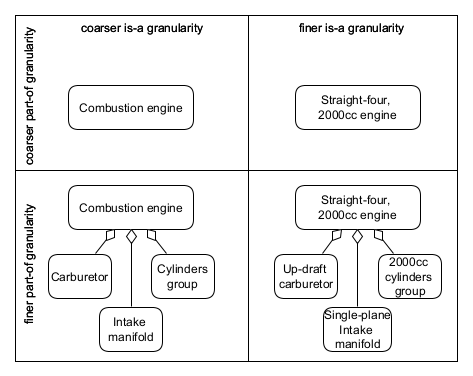
\includegraphics[width=\textwidth]{2-ways-granularity-table-new-new.PNG}
    %\caption{A simplified structural model of a combustion engine. Starting from the engine as a whole one can go towards a finer mereological-granularity and find out that the engine is made of three components; going towards a finer subsumption-granularity one can find out that the engine is not just an instance of any combustion engine, but has additional properties (in this case the number, location, and volume of the cylinders), and the same holds fro the engine parts.}
    \caption{}
    \label{fig:2-ways-granularity-table-new-new}
    \end{subfigure}
    \hfill
    \begin{subfigure}{0.40\textwidth}
%    \centering
    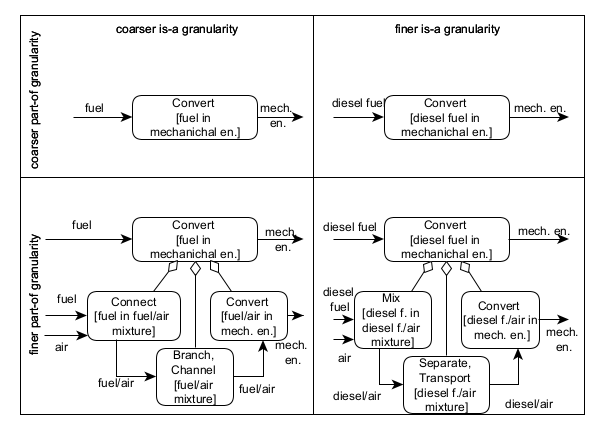
\includegraphics[width=\textwidth]{2-ways-granularity-table-functions.png}
    %\caption{\label{fig:2-ways-granularity-table-function}A simplified functional model of a combustion engine using the Functional Basis methodology. For simplicity, we refer to the structure in Figure \ref{fig:2-ways-granularity-table-new-new} and assume that each part of a system has a function. Using the Functional Basis vocabulary, the function of the engine could converting fuel into mechanical energy, while the function of carburetor is to mix fuel and air, and so on for the other components. In this case, moving to a finer granularity level over the aggregation relation means decomposing the current function, while moving to a finer granularity level on the is-a relation is achieved by moving to a finer level of the functions vocabulary (e.g, from `connect' to `mix'), as well as using more precise terms for the flows.}
    \caption{}
    \label{fig:2-ways-granularity-table-function}
    \end{subfigure}
\caption{\subref{fig:2-ways-granularity-table-new-new}: A simplified structural model of a combustion engine. Starting from the engine as a whole one can go towards a finer mereological-granularity and find out that the engine is made of three components; going towards a finer subsumption-granularity one can find out that the engine is not just an instance of any combustion engine, but has additional properties (in this case the number, location, and volume of the cylinders), and the same holds for the engine parts. \\
\subref{fig:2-ways-granularity-table-function}: A simplified functional model of a combustion engine using the Functional Basis methodology. For simplicity, we refer to the structure in Figure \subref{fig:2-ways-granularity-table-new-new} and assume that each part of a system has a function. Using the Functional Basis vocabulary, the function of the engine is converting fuel into mechanical energy, while the function of carburetor is to mix fuel and air, and so on for the other components. In this case, moving to a finer granularity level over the aggregation relation means decomposing the current function, while moving to a finer granularity level on the is-a relation is achieved by moving to a finer level of the function vocabulary (e.g, from `connect' to `mix'), as well as using more precise terms for the flows.}
\label{fig:due-figure}
\end{figure}

%We are especially interested in the case that it is the relation is the one 


% Functional decomposition is essential, because of multiple reasons. We lists some of those in the following (some points refers to the structural hierarchy and not to the functional one, but, if we assume that some relation exists between the physical components of a system and its functions, they translate to the functional hyerarchy as well):

Granularity is important when modelling engineering systems for, at least, the following reasons:
\begin{itemize}
    \item \textbf{Accounting for different viewpoints.} Different operations carried out on a product during the various step of its lifecycle require different points of view about the product. Those viewpoints may differ also due to the level of granularity they focus on, for example, during the assembly of a machine, a car say, it may be very important for the workers to know where each screw goes and what kind of washer is required. On the other hand, during maintenance, it may happen that, if a part of the car is malfunctioning, it is simply replaced as a whole.%, and no diagnostic is carried out to determine what was wrong within that part, because it would be too costly in time and money, even if that part was assemblied by the same company that is carrying out maintenance. 
    \item \textbf{Simplifying the management of complex systems.} Engineered systems can be extremely complex, and when that happens it would be very difficult to manage them using a fixed level of granularity. This is because that level would necessarily be the finest one, otherwise some information would be lost. But this would be akin to always treat a complex system, say a car, as a list of screws, bolts, pipes, metal plates and pieces of various shapes, etc., which would be untenable. \TODO{<--FC: remove last 2 sentences for conciseness?}
    \item \textbf{Reasoning about engineering systems.} Human reasoning about engineering systems often requires jumping between different levels of granularities. For example, the German school of systematic design \cite{pahl_engineering_2007} explicitly describes the design process as the development of a functional hierarchy (`funktionsstruktur') starting from the coarsest level of granularity (the main function the product to be designed should satisfy) and going down to finer-granularity-level functions until one reaches a point that can be readily translated to an assembly of physical items (`embodyment' of the functions). Analogously, a common way for technicians to troubleshoot a malfunctioning system is to produce a chain of parts, each one `containing' the malfunction and strict subpart of the proceeding part. %The method used to isolate the next part of the sequence vary, but it could very well be based on function of the part (e.g., if a laptop is not playing music correctly the problem will be -- among other possibilities -- in its speakers; if, more precisely, the music is played always too softly, the problem will be in the amplifying circuit within the speakers, etc.)
    \item \textbf{Allowing scalability of applications.} Suppose that one were to build a simplified model of some system as a proof-of-concept, and some application is developed to interact with such a model. Later, if this system is implemented, the actual model may become orders of magnitude bigger than the preliminary one. If the behaviour of the application concerning granularity was not well thought out, it may happen that the application malfunctions with the full model.    
\end{itemize}

We are especially interested in the granularity of aggregation-like\footnote{Again, we cannot assume in general that the relation is a part-whole relation \cite{vermaasFormalImpossibilityAnalysing2013}.} relations between functions (that is, a functional decomposition), to facilitate the previous points achieving a solution to Problem \refpb{granularity-problem}. Moreover, functional modelling is seldom used in actual engineering practice, despite its emphasis in the literature; we believe that effective management of granularity is instrumental in facilitating functional modelling adoption by engineering enterprises.

Also in this case we argue in favour of a particular style of decomposition, among the few possibilities described in Section \ref{sec:literature} (the following considerations can be applied \textit{mutata mutatis} to other functional theories):

\begin{itemize}
  \item \textbf{Functional Basis style of decomposition.} This style of decompositions was briefly described in Section \ref{sec:literature}, see also Figure \ref{fig:2-ways-granularity-table-function}. We argue that this style of decomposition has some weak points:
  \begin{itemize}
    \item It is not (intrinsically) modular: decomposition happens by substituting a box with some input and output flows with a set of boxes with additional flows between them (the original in/out flows are preserved). It may be possible to, say, label some typical decompositions and reuse them, but this is not discussed in the literature on the Functional Basis \TODO{check}, even though some works of the German School of systematic design (e.g. \cite{rothKonstruierenMitKonstruktionskatalogen2000}), which the Functional Basis is based on, go, essentially, in that direction. 
    \item At a fine level of granularity, the decomposition of a system, say an electrical or hydraulic system, becomes redundant with the electric or hydraulic schematics already commonly used by engineers. This is intended, since this methodology aims to produce, at the end of the design process, a decomposition that is readily translatable in such schematics. Since we want to focus (at least) on maintenance activities, we assume that such schematics already exist, therefore, the decomposition from a functional point of view would be redundant. Moreover, it is generally considered useful that functional and structural representations are independent (see e.g. \cite{ISOIEC8134612009}).
    \item The function taxonomy is just three levels deep. This presumably, helps with systematicity, but it imposes only three subsumption-granularity levels (e.g., we cannot distinguish between cooling or heating).
  \end{itemize}
  \item \textbf{Functional Representation style of decomposition.} This style is modular by design: we just need to label some CDPs and reuse them. On the other hand, the functions are not organized in a taxonomy, except for the four types determined by Keuneke \cite{keuneke_device_1991}. Moreover, the reduction of functions as labels for state transitions makes it so that, at fine granularity levels, the decomposition becomes a sort of a behavioural diagram, which could be even used to simulate the system as a finite state machine. This may fit some applications, but, again, it does not limit itself to only teleological aspects.
  \item \textbf{FBRL style of decomposition.} This style is also modular by design: in this case the `way-of-achievements' can be reused. Additionally, function-classes are organized in a rich taxonomy \TODO{citaz}; even the `way-of-achievements' are organized in rich taxonomies which implement domain-specific knowledge\TODO{citaz}. Finally, this methodology introduces also teleological relations between functions (`meta-functions') which, arguably, allow the decomposition to stay on a purely teleological level. 
\end{itemize}
In Section \ref{sec:use-case} we will showcase a simplified application of our interpretation of FBRL-style functional decomposition.

%\subsection{Malfunction}\TODO{S: lascerei questo argomento per un articolo successivo [FC: my thoughts, exactly]}
%We touch this topic only briefly, since a full discussion is outside the scope of this paper.
%\TODO{<spiegare principali classificazioni relative a guasti e argomentare che la divisione in funzioni ontolo./sist./ing.-metodi riflette un'analoga suddivisione a livelli di guasti, che è originale e interessante> delete? This is waaay out of space.}

\section{Examplification}\label{sec:use-case}

Here we very briefly outline how to implement, in a conceptual model, some of the previous considerations.

First, we need a taxonomy accomodating both physical objects and functions. Figure \ref{fig:class-taxonomy} show a DOLCE-based \cite{borgoDOLCEDescriptiveOntology2022} putative taxonomy of such a kind, which subsumes functions into a category for role-concepts, and%, based on previous work \TODO{si può citare un lavoro che ancora non si sa se ha passato la revisione? Immagino di no, però sarebbe duopo.} \TODO{The characteristic feature is the high-level categorisation of functions in three classes: ontological, systemic, and engineering functions, as well as a separate [...] <--FC:rimuovere}
supplies a separate category for `way-of-achievements' (called engineering methods), which can then be specialized into different function- and method-kinds. These classes should be characterised ontologically, but this is outside the scope of this paper and we delegate it to further research work. \TODO{<--FC:skippato l'articolo per SWJ}

Then, a functional decomposition of an engineering system can be achieved, alternating between methods and functions. Figure \ref{fig:functional-decomposition} shows an implementation of this, to decompose the function of a steady rest of a laser cutting machine.
Such a machine cuts metal tubes using a laser beam emitted from a mobile cutting head. The tubes are moved by a spindle that rotates and translates. In order to increase the quality of the cut, the workpiece must be kept in place very precisely. To do this, a specific apparatus, called \textit{steady rest} is used. Since steady rests are commonly used in tooling machines, not only in laser cutting machines, they are implemented as a known engineering method. In this particular case, the steady rest is automated, therefore some method must be selected to allow it \textit{to rotate}, among other things. Thus, the decomposition employs the common method to use an \textit{electrical motor} (together with typical auxillary parts such as a gearbox and a pinion-crown gear coupling). This method can be further divided into a \textit{conversion of electrical energy into mechanical energy} function, realized by the motor proper, and a \textit{transmit mechanical energy} function, realized by the gears and shafts linked to the motor. The decomposition can go on, until the desired granularity level is reached. 
Notice that this functional decomposition manages granularity well, in the sense that it is easy to build deep trees; and is modular, as, for example, the motor-gearbox-pinion and the hydraulic cilynder methods will be reused many times in the tree.

Finally, as explained in Section \ref{subsec:identity}, replacement of parts can be modelled, by making use of the functional roles as constant `anchors' for the replaced physical objects. It suffices just a link between physical objects and functions, together with, for example, attributing to the physical objects the times of installation and removal from the system. Figure \ref{fig:replacement} shows such an example: two motors are installed in the same system, at different times, at the same `functional location' (here interpreted as simply some fixed function).

\begin{figure}
  \centering
  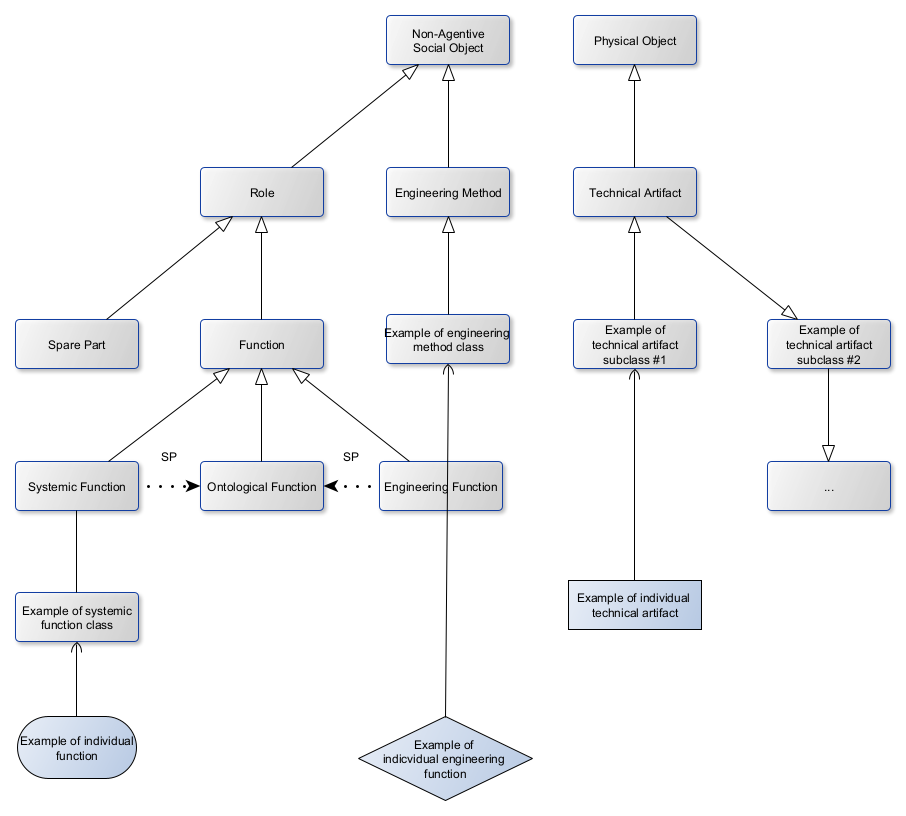
\includegraphics[width=0.50\textwidth]{class-taxonomy.png}
  \caption{\label{fig:class-taxonomy}}
\end{figure}
\begin{figure}
  \centering
  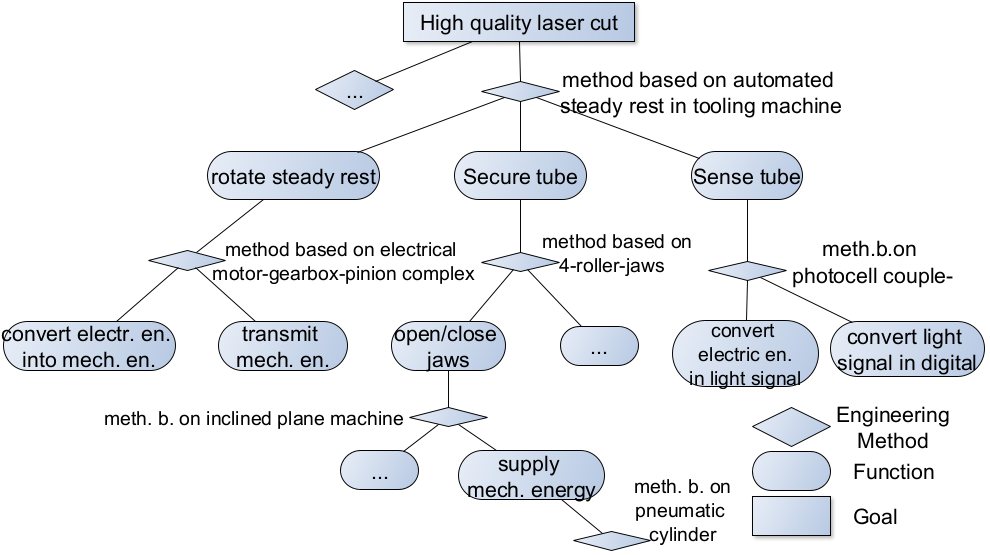
\includegraphics[width=0.80\textwidth]{functional-decomposition.png}
  \caption{\label{fig:functional-decomposition}}
\end{figure}
\begin{figure}
  \centering
  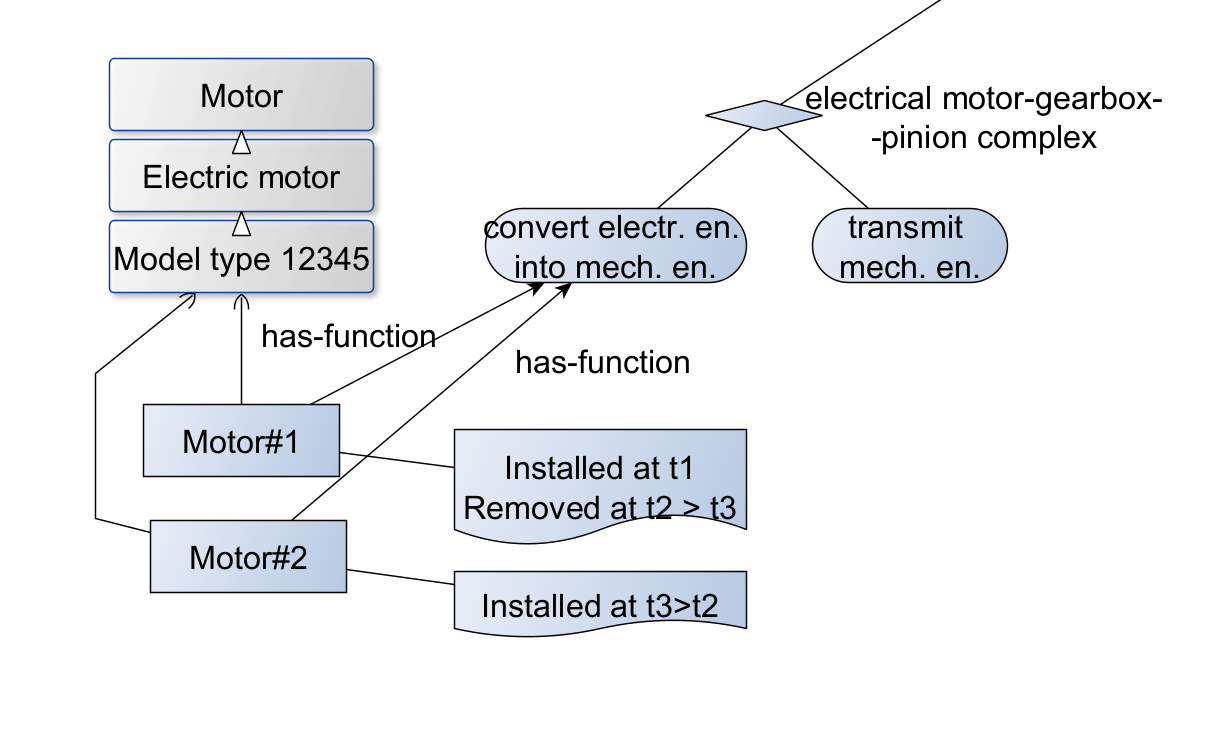
\includegraphics[width=0.40\textwidth]{functional-decomposition-with-replacement.png}
  \caption{\label{fig:replacement}}
\end{figure}

\section{Conclusion}
We have summarily described two recurring problems in functional modelling, and used ontological arguments to characterise some of the most common methodologies used in functional modelling with respect to these problems.
Finally, we have suggested an effective way to manage these problems and we have very briefly shown how it can be implemented in conceptual modelling.

\acknowledgments

\TODO{Francesco Compagno is funded by the company Adige Spa. This work is partially funded by the European project
OntoCommons (GA 958371, www.ontocommons.eu).
}



\bibliography{biblio-funzioni}

\end{document}

%% MEMO CITAZIONI 

% What is a functional location?
% `[In the context of] Plant Maintenance, 
% An organizational unit in Logistics that structures the maintenance objects of a company according to functional, process-oriented, or spatial criteria. A functional location represents the place at which a maintenance task is performed.' Notice that, despite the name, the spatial criteria is only one possible criteria for identifying the functional location.
% \url{https://help.sap.com/glossary/?locale=en-US&term=functional%2520location} accessed May 2022.


% `ISO 15926-14 includes terms for defining restrictions identified in the design phase and terms for the transition from design to procurement. This includes in particular class terms for physical objects, systems, functions and functional objects. 

% Using these terms one can capture the evolution of functional objects from an early design phase to the functional locations of tag numbers and capture the distinction between a tag number and a physical object installed at the tag. This feature is exploited in the modelling patterns for lifecycle information.' --page 11

% `The starting point is a system s, with functional parts a and b represented by the object property functionalPartOf. Both the system s and its functional parts a and b are classified as FunctionalObject. A functional object could be a tag, or an object identified in the design process at a point before tags are introduced.' --page 60

% `An important point is that the breakdown structure of the physical objects may be very different from the system breakdown structure captured by the object property functionalPartOf. The physical breakdown structure is not illustrated, but could be captured by part/whole properties, e.g., arrangedPartOf.' --page 61

% `The story begins with the creation of a functional object that fulfills the need for pumping. The object is then associated with Function Requirements (FR) specifying such details as rated power, etc. Next, the location for the object is specified as well as the Component Type (CT) and a Product Specification (PS) is given. Once the specifications are in place, an actual motor, i.e. a physical object, is installed and, later, replaced by another motor as part of a maintenance policy.' -- page 65

% `Class: lis:System Annotations: rdfs:comment "A system is a complex of functional parts working together. Each part contributes to the realisation of the system's function (though not necessarily every part in every performance of the system).", rdfs:label "System", skos:note "A functional location that does not itself have functional parts is not a system.",' --annex F

% functional locations are implicitly equiparated to functional objects, see Figure G.5.3.

% `Class: lis:FunctionalObject Annotations: rdfs:comment "A functional object is part of a system, and has a function whose realisation contributes to the performance of the system as a whole.", rdfs:label "FunctionalObject", skos:example "An item on a Process Flow Diagram (PFD) or Process and Instrumentation Diagram (P\&ID) should be classified as a FunctionalObject.", skos:note "A class of artefacts such as Pump is not a subclass of FunctionalObject: a pump that is not in service is not part of a system. However, an individual functional location should in general be given some high-level artefact classification in addition to its description as part of a system.", skos:prefLabel "FunctionalObject" SubClassOf: lis:Object, lis:functionalPartOf some lis:System, lis:hasFunction some lis:Function Every object in an industrial plant is there for a purpose, and the objects are arranged into systems of “functional objects”. Plant design assigns one or more functions to each functional object'--page 20[10]